\section{Methodology}

\subsection{Profiling}
When making an effort to accelerate a model like DALES, one should first figure out which parts of the code contribute the most to the wall clock time. This act is called profiling, and there are numerous tools available that serve this purpose. One tool in particular that is very well suited for GPU applications, is NVIDIA's Nsight Systems (NSys) \citep{nvidiaNVIDIANsightSystems}. NSys automatically tracks CPU-GPU interactions, such as data transfer, and GPU utilization, but does not track CPU utilization. To track CPU activity, a custom timer module based on the NVIDIA Tools Extension (NVTX) library is used, allowing the programmer to annotate sections of their code to measure their wall-clock time. NSys comes with a GUI to visually inspect the profile (\autoref{fig:nsys}). NSys will be used to track performance and data locality.

\begin{figure}[H]
    \centering
    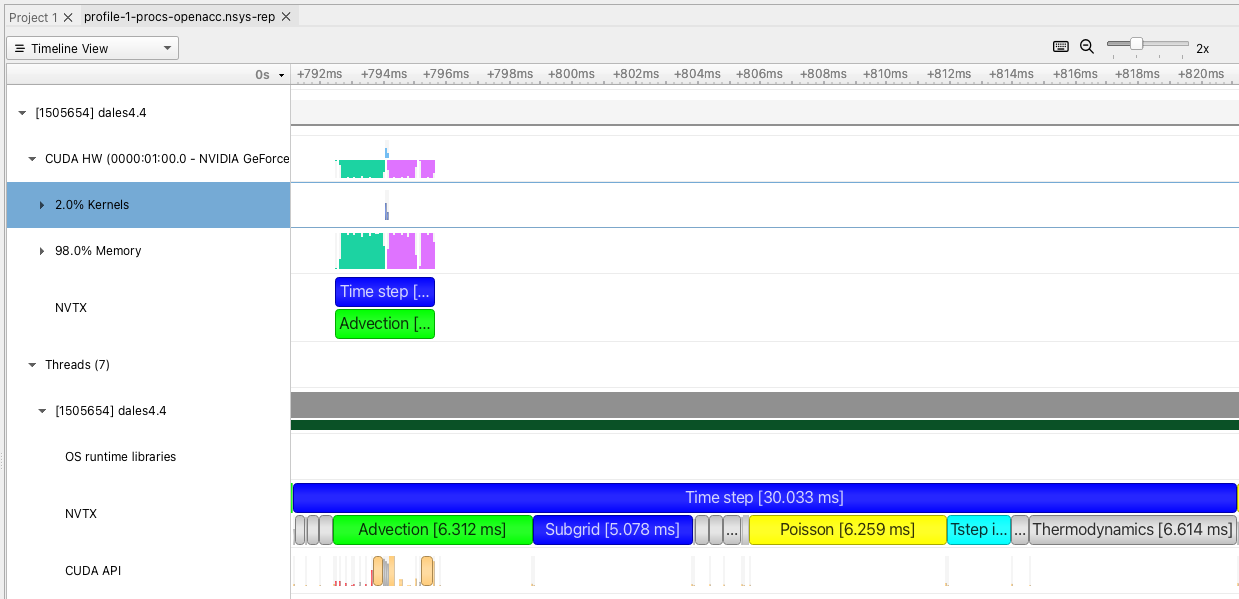
\includegraphics[width=0.9\textwidth]{doc/images/profiles/nsys.png}
    \caption{A screenshot of the NSys GUI. The main subroutine calls in DALES' time steps have been annotated with NVTX markers and show up at the bottom of the image, with their execution time between brackets. To demonstrate the GPU tracking capabilites of NSys, one advection kernel has been offloaded to the GPU (\texttt{advecu\_2nd}), which shows up under ``CUDA HW''. It can be seen that NSys automatically separates kernel execution time from time spent on memory operations, allowing for easy identification of performance bottlenecks.}
    \label{fig:nsys}
\end{figure}

\subsection{OpenACC}
As concluded from the literature, OpenACC is a relatively easy model to implement into an existing code base, while still offering good performance, given that data locality is properly optimized. Hence, the computationally expensive parts of DALES will be offloaded to the GPU using OpenACC. In \autoref{fig:nsys}, it can be seen that during one time step, most time is spent on the advection, sub-grid, Poisson and thermodynamics modules. These modules are expensive, because they consist mostly of loops that iterate over all grid points, making them also very well suited for offloading to GPUs with OpenACC. 

The first step in getting DALES running on GPUs, is to place OpenACC directives over all loops that are parallelizable. An example of a loop with an OpenACC directive can be found in \autoref{listing:accloop}. This will be done one module at a time. 

\begin{listing}[H]
\begin{minted}{fortran}
!$acc parallel loop
do k = 1, kmax
    do j = 1, jmax
        do i = 1, imax
            c(i,j,k) = a(i,j,k) + b(i,j,k)
        end do
    end do
end do
\end{minted}
\caption{Example of a Fortran loop decorated with an OpenACC directive. The directive \texttt{!\$acc parallel loop} tells the compiler that the following loop can be executed in parallel}
\label{listing:accloop}
\end{listing}

\subsection{Solving the Poisson equation}

In DALES, a solution for the pressure $\pi$ is obtained by solving the following Poisson equation:

\begin{equation}
    \frac{\partial^2 \pi}{\partial x_i^2} = \frac{\partial }{\partial x_i} \left( - \frac{\partial \overline{u}_i \overline{u}_j}{\partial x_j} + \frac{g}{\theta_0}\overline{\theta}_v\delta_{i3} + \mathcal{F}_i - \frac{\partial \tau_{ij}}{\partial x_j} \right) \label{eq:pressure}
\end{equation}

 DALES provides two methods to solve this equation: using Fast Fourier Transforms (FFT's), or using iterative solvers. Among these, the FFT-based solver is the fastest. DALES has the ability to use the highly optimized Fastest Fourier Transform in the West (FFTW) library \citep{FFTW97}. FFTW is not capable of running on GPU's, however. NVIDIA provides a FFT library in their HPC SDK, which has a similiar interface as the FFTW library, making the conversion relatively straightforward. Consequently, the hand-coded transpose subroutines have to be adopted for the GPU as well. Alternatively, the multi-process version of cuFFT, cuFFTMp, can used. This library enables multi-process, multi-GPU FFTs, without the need to transpose the data and perform \texttt{MPI\_Alltoall} manually. In fact, inter-GPU communication is optimized using another communication library called NVSHMEM ,  The cuFFTMp libary can bind to an existing MPI Communicator, and handle communications between GPUs by itself. Yet another option is to use the cuDecomp library as described by \citet{romeroDistributedmemorySimulationsTurbulent2022}. Similar to cuFFTMp, cuDecomp 

\subsection{Verification}
Modifying source code brings the possibility of introducing bugs in the code. While OpenACC requires minimal rewriting of source code, some rewriting may be inevitable. Hence, the updated source code needs to be validated against the original, unmodified code to check whether the program logic has changed. To this end, one would usually assert whether the end result of the two programs are equal or not. This approach is not feasible for a simulation of a turbulent boundary layer, however, as weather-like simulations are subject to chaos. A small perturbation of some prognostic variable can lead to vastly different results in the end. One source of such a perturbation can be the rounding off done by the computer. Even when using the exact same initial conditions, the point-wise end results of two runs may still differ, while each of the solutions could still be considered correct. A better approach would be to look at averaged statistics of several variables. 

